\documentclass[../main.tex]{subfiles}

\begin{document}

\section{Conjuntos}
\subsection{¿Qué es un conjunto?}
Un conjunto corresponde a una colección bien definida de objetos. Estos objetos son denominados como \textbf{elementos del conjunto} y se dice que estos \textbf{pertenecen} (expresado con el simbolo $\in$) a él.\\
Cuando definimos un conjunto, se usan símbolos de llaves y dentro se colocan todos los objetos que pertenecen al conjunto.\\
Ejemplo:
\[ S = \{ 1, 2, 3, 4 \} \]

\subsection{Nociones básicas de los conjuntos}
\subsubsection{Pertenencia ($\in$)}
Si tenemos un conjunto $S$ y un objeto $a$, se dice que
\begin{itemize}
    \item $a \in S$ cuando el objeto $a$ se encuentra dentro del conjunto S.
    \item $a \not\in S$ cuando el objeto $a$ \textbf{no} se encuentra dentro del conjunto S.
\end{itemize}
\textbf{NOTA:} Un objeto puede ser un conjunto. Esto significa que un conjunto puede pertenecer a otro conjunto.

\subsubsection{Subconjunto ($\subseteq$)}
Considerando a un conjunto $A$ y un conjunto $B$, se dice que $A$ es subconjunto de $B$ si
\[ \forall x . x \in A \rightarrow x \in B \]
En otras palabras, $A$ es subconjunto de $B$ si todo elemento presente en $A$ está presente en $B$ también. Cuando esto ocurre, se denota como $A \subseteq B$ (y cuando no, lógicamente se escribe como $A \not\subseteq B$)

\subsubsection{Igualdad de conjuntos}
Diremos que dos conjuntos $A$ y $B$ son iguales si se cumple que
\[ A \subseteq B \wedge B \subseteq A \quad \text{o, escrito de otra forma} \quad \forall x . x \in A \leftrightarrow x \in B \]
En palabras simples, dos conjuntos son iguales cuando ambos conjuntos tienen exactamente los mismos objetos, sin ninguno que pertenezca a un conjunto y no a otro. Esto se expresa como $A = B$ (y cuando no, $A \not= B$).

\subsubsection{Conjunto vacío}
Existe un conjunto único $\emptyset$, el cual llamamos \textit{conjunto vacío}, el cual cumple que 
\[ \forall x . x \not\in \emptyset \]

\subsection{Descripción de un conjunto}
\begin{enumerate}
    \item Por extensión: Este es el método más básico y el cual se describió anteriormente. Simplemente se listan todos los contenidos del conjunto entre llaves.\\
    Ejemplo: \[ S = \{ 1, 2, 3, 4 \} \]
    \item Por comprensión: Se define una propiedad $\delta(x)$ en algún lenguaje formal que solo cumplen los elementos del conjunto.\\
    Ejemplo: \[ S = \{ x | \delta(x) \text{ es verdadero} \} \]
    Ejemplo un poco más creativo: \[ P = \{ x | \forall x . x \text{ es par} \} \]
\end{enumerate}

\subsection{Paradoja de Russell o Paradoja del Barbero (1901)}
\begin{wrapfigure}{r}{0.25\textwidth}
    \centering
    
\includegraphics[width = 0.25\textwidth]{b_russell.png}
    \text{B. Russell (1872 - 1970)}
\end{wrapfigure}
Esta es una paradoja enunciada por Bertrand Russell\footnote{Esta sección contiene información extraída del \href{https://es.wikipedia.org/wiki/Paradoja_de_Russell}{siguiente artículo de Wikipedia}.}. Para comenzar, se define el siguiente conjunto
\[ S^* = \{ B \  | \  B \not\in B \} \]
$S^*$ corresponde al ``conjunto de todos los conjuntos que no se contienen a si mismos como miembros''. Ahora, recordemos que por la definición de lo que es un conjunto, esto es equivalente a
\[ \forall B . B \in S^* \leftrightarrow B \not\in B \]
O sea, ``cada conjunto es elemento de $B$ si y solo si no es elemento de si mismo''. Debido a que $B$ es un conjunto, lo podemos sustituir de la siguiente forma
\[ S^* \in S^* \leftrightarrow S^* \not\in S^* \]
lo cual es una contradicción.\\
Esto puede ser un poco complicado de entender así. Intentemos entenderlo con la historia del Barbero.

\includegraphics[width = 0.5\textwidth]{barb_1.png}
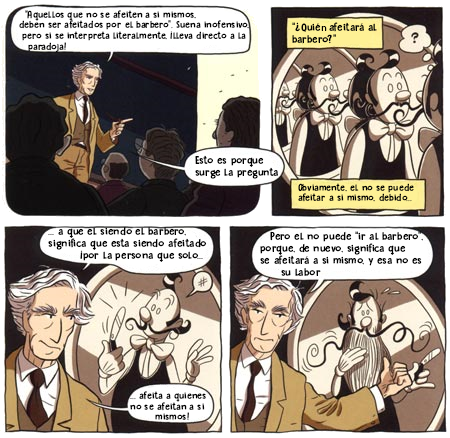
\includegraphics[width = 0.5\textwidth]{barb_2.png}

Una definición como esta es bastante problemática. El problema aquí es \textit{``considerar definiciones que se referencian a si mismas''}. Esto nos deja de lección que no todas las definiciones son válidas en la teoría de conjuntos.\footnote{Todas las definiciones que se verán durante el curso son válidas, pero esto es una lección de que no siempre es así.}

\subsection{Operaciones sobre conjuntos}
\begin{itemize}
    \item Unión ($\cup$): $A \cup B$ son todos los elementos que se encuentran en $A$ o en $B$.
    \[ A \cup B = \{ x | x \in A \vee x \in B \} \]
    \item Intersección ($\cap$): $A \cap B$ son todos los elementos que se encuentran en $A$ y $B$ al mismo tiempo.
    \[ A \cap B = \{ x | x \in A \wedge x \in B \} \]
    \item Diferencia ($\backslash$): $A \backslash B$ son todos los elementos que se encuentran en $A$ y no en $B$.
    \[ A \backslash B = \{ x | x \in A \wedge x \not\in B \} \]
    \item Complemento ($A^C$): $A^C$ corresponde a todos los elementos que no se encuentran en $A$.
    \[ A^C = \{ x | x \not\in A\} \]
\end{itemize}

\subsubsection{Propiedades de las operaciones sobre conjuntos}
Para conjuntos $A$, $B$ y $C$ y un universo $\mathcal{U}$ tenemos las siguientes propiedades
\begin{enumerate}
    \item Asociatividad:
    \[
        \begin{tabular}{rcl}
            $A \cup (B \cup C)$ & $=$ & $(A \cup B) \cup C$ \\
            $A \cap (B \cap C)$ & $=$ & $(A \cap B) \cap C$ \\
        \end{tabular}
    \]
    \item Conmutatividad:
    \[
        \begin{tabular}{rcl}
            $A \cup B$ & $=$ & $B \cup A$ \\
            $A \cap B$ & $=$ & $B \cap A$ \\
        \end{tabular}
    \]
    \item Idempotencia:
    \[
        \begin{tabular}{rcl}
            $A \cup A$ & $=$ & $A$ \\
            $A \cap A$ & $=$ & $A$ \\
        \end{tabular}
    \]
    \item Absorción:
    \[
        \begin{tabular}{rcl}
            $A \cup (A \cap B)$ & $=$ & $A$ \\
            $A \cap (A \cup B)$ & $=$ & $A$ \\
        \end{tabular}
    \]
    \item Distributividad:
    \[
        \begin{tabular}{rcl}
            $A \cup (B \cap C)$ & $=$ & $(A \cup B) \cap (A \cup C)$ \\
            $A \cap (B \cup C)$ & $=$ & $(A \cap B) \cup (A \cap C)$ \\
        \end{tabular}
    \]
    \item De Morgan
    \[
        \begin{tabular}{rcl}
            $(A \cup B)^C$ & $=$ & $A^C \cap B^C$ \\
            $(A \cap B)^C$ & $=$ & $A^C \cup B^C$ \\
        \end{tabular}
    \]
    \item Elemento neutro:
    \[
        \begin{tabular}{rcl}
            $A \cup \emptyset$ & $=$ & $A$ \\
            $A \cap \mathcal{U}$ & $=$ & $A$ \\
        \end{tabular}
    \]
    \item Dominación:
    \[
        \begin{tabular}{rcl}
            $A \cap \emptyset$ & $=$ & $\emptyset$ \\
            $A \cup \mathcal{U}$ & $=$ & $\mathcal{U}$ \\
        \end{tabular}
    \]
    \item Elemento inverso:
    \[
        \begin{tabular}{rcl}
            $A \cup A^C$ & $=$ & $\mathcal{U}$ \\
            $A \cap A^C$ & $=$ & $\emptyset$ \\
        \end{tabular}
    \]
\end{enumerate}

\subsubsection{Paréntesis y precedencia}
Se asumirá el siguiente orden de precedencia entre operadores
\[
    \begin{tabular}{cc}
        Operadores & Precedencia \\ \hline
        $.^C$ & $1$ \\
        $\cap$ & $2$ \\
        $\cup$ & $3$
        
    \end{tabular}
\]

\subsubsection{Operaciones generalizadas}
\begin{itemize}
    \item Unión generalizada: $\bigcup \mathcal{S}$ son todos los elementos que pertenecen a algún elemento de $\mathcal{S}$.
    \[ \bigcup \mathcal{S} = \{ x \  | \ \exists A .\  A \in \mathcal{S} \wedge x \in A \} = \bigcup_{A \in \mathcal{S}} A = \bigcup_{i = 1}^{k} A_i \]
    \item Intersección generalizada: $\bigcap \mathcal{S}$ son todos los elementos que pertenecen a todos los elementos de $\mathcal{S}$
    \[ \bigcap \mathcal{S} = \{ x \  | \ \forall A .\  A \in \mathcal{S} \rightarrow x \in A \} = \bigcap_{A \in \mathcal{S}} A = \bigcap_{i = 1}^{k} A_i \]
\end{itemize}

\subsection{Conjunto Potencia}
Para un conjunto $A$, el conjunto potencia $\mathcal{P}(A)$ de todos los subconjuntos de $A$ es definido como:
\[ \mathcal{P}(A) = \{ X \  | \  X \subseteq A \} \]
En palabras simples, el conjunto potencia de $A$ corresponde al conjunto que contiene a todos los subconjuntos de $A$.\\

\subsection{Cardinalidad de un conjunto}
La cardinalidad del conjunto corresponde a la cantidad de elementos distintos contenidos en un conjunto
\[ A = \text{\# de elementos distintos en } A \]
\textbf{Teorema:}
\[ A = \{ 1, 2, 3, \ldots, n \} \rightarrow |\mathcal{P}(A)| = 2^n \]
En otras palabras, la cardinalidad del conjunto potencia de $A$ corresponde a 2 elevado a la cardinalidad del conjunto $A$.

\subsection{Grafos como conjuntos}
Pero \ldots ¿qué es un grafo?\footnote{Información extraida del siguiente \href{https://es.wikipedia.org/wiki/Grafo}{artículo de Wikipedia}}\\
Un grafo consiste en un conjunto de objetos llamados vertices y nodos, los cuales se encuentran unidos entre sí.\\
\textbf{Definición:} Un grafo $G$ sobre el dominio $V$ es un subconjunto $E \subseteq \mathcal{P}(V)$, tal que para todo $e \in E$ se cumple que $|e| = 2$.
\[
    \begin{tikzpicture}[roundnode/.style={circle, draw=black!60, very thick, minimum size=7mm}]
        %Nodos
        \node[roundnode] (a) {a};
        \node[roundnode] (b) [right=of a] {b};
        \node[roundnode] (c) [below=of a] {c};
        \node[roundnode] (d) [right=of c] {d};
        \node[roundnode] (e) [right=of b] {e};
        \node[roundnode] (f) [right=of d] {f};
        \node[roundnode] (g) [above=of e] {g};
        %Lineas
        \draw (a) -- (b);
        \draw (a) -- (d);
        \draw (a) -- (c);
        \draw (b) -- (e);
        \draw (c) -- (d);
        \draw (d) -- (e);
        \draw (d) -- (f);
        \draw (e) -- (g);
        \draw (f) -- (e);
        \draw (a) -- (g);
    \end{tikzpicture}
\]
\[
    \begin{tabular}{rcl}
        $V$ & = & \{a, b, c, d, e, f, g\}\\
        $E$ & = & \{ \{a,b\}, \{a,c\}, \{a,d\}, \{a,g\}, \{b,e\}, \{c,d\}, \{d,e\}, \{d,f\}, \{e,f\}, \{e,g\} \}\\
    \end{tabular}
\]
En un grafo, los elementos que están presentes en $V$ los llamamos \textit{vértices o nodos}, y los elementos en $E$ los llamamos \textit{aristas}.

\subsection{Pares Ordenados}
Para dos elementos $a$ y $b$ se define el par ordenado $(a,b)$ como
\[ (a,b) = \{ \{ a \}, \{ a,b \} \} \]
De forma mas informal, decimos que $(a,b)$ es un par ordenado si es que el primer elemento ($a$) se distingue del segundo elemento ($b$). Por esto, tenemos que $(a,b) \not= (b,a)$.\\
\textbf{Generalización:} Se define una \textit{n-tupla ordenada} como
\[ (a_1, a_2, \ldots, a_n) = ((a_1, a_2, \ldots, a_{n-1}), a_n) \]

\subsection{Producto Cartesiano}
Sea $A$ y $B$ conjuntos. El producto cartesiano se define como
\[ A \times B = \{ (a,b) \  | \  a \in A \wedge b \in B \} \]
Si tenemos $n$ conjuntos $A_1, A_2, \ldots, A_n$, el producto cartesiano generalizado es
\[ A_1 \times A_2 \times \ldots \times A_n = \{ (a_1, \ldots, a_n) \  | \ a_i \in A_i \} \]

\section{Relaciones}
Considerando un conjunto $A$ y $B$, $R$ es una relación binaria sobre $A$ y $B$ si se cumple que
\[ R \subseteq A \times B \]
Es posible que $B = A$, entonces se dice que $R$ es una relación binaria sobre $A$
\[ R \subseteq A \times A \]
\textbf{Notación:} Para una relación $R$ y un par $(a,b)$, se usará la siguiente notación\\
\[
    \left.
        \begin{array}{c}
            (a,b) \in R \\
            \text{o} \\
            a \ R \ b
        \end{array}
    \right	
        \} \quad (a, b) \text{ pertenece a la relación } R
\]

\declareslashed{}{/}{0.05}{0}{R}

\[
    \left.
        \begin{array}{c}
            (a,b) \not\in R \\
            \text{o}\\
            a \ \slashed{R} \ b
        \end{array}
    \right
        \} \quad (a,b) \text{ no pertenece a la relación } R
\]

\subsection{Representación de Relaciones}
\subsubsection{Grafos dirigidos}
Toda relación binaria $R$ sobre $A$ se puede ver como un grafo dirigido $G_R = (A,R)$\\
Ejemplo:
\[ A = \{ a, b, c, d, e \} \quad ; \quad R = \{ (a,b), (b,b), (c,b), (c,d), (d,a), (d,d), (d,e) \} \]
\[
    \begin{tikzpicture}[roundnode/.style={circle, draw=black!60, very thick, minimum size=7mm}]
        %Nodos
        \node[roundnode] (a) {a};
        \node[roundnode] (b) [right=of a] {b};
        \node[roundnode] (c) [below=of a] {c};
        \node[roundnode] (d) [right=of c] {d};
        \node[roundnode] (e) [right=of d] {e};
        %Lineas
        \draw [-stealth] (a) -- (b);
        \draw [-stealth] (c) -- (b);
        \draw [-stealth] (c) -- (d);
        \draw [-stealth] (d) -- (e);
        \draw [-stealth] (d) -- (a);
        \draw [-stealth] (b) to[out=30, in=-30, looseness=4] (b);

    \end{tikzpicture}
\]

\subsubsection{Matrices sobre bits / Representación Matricial}
Sea $A = \{ a_1, a_2, \ldots, a_n \}$ un conjunto y $R$ una relación binaria sobre $A$. Definimos la matriz $M_R$ que representa a la relación $R$ como
\[ M_R[i, j] = 
    \begin{cases}
        1 & \text{si} \; a_i \ R \ a_j\\
        0 & \text{si} \;  a_i \ \slashed{R} \ a_j
    \end{cases} 
\]
Ejemplo:
\[ A = \{ a, b, c, d, e \} \quad ; \quad R = \{ (a,b), (b,b), (c,b), (c,d), (d,a), (d,d), (d,e) \} \]
\[
    \left.
        \begin{bmatrix}
            0 & 1 & 0 & 0 & 0\\
            0 & 1 & 0 & 0 & 0\\
            0 & 1 & 0 & 1 & 0\\
            1 & 0 & 0 & 1 & 1\\
            0 & 0 & 0 & 0 & 0\\
        \end{bmatrix}
    \right. \hspace{3em}\raisebox{-3em}{
        \begin{tikzpicture}[roundnode/.style={circle, draw=black!60, very thick, minimum size=7mm}]
            %Nodos
            \node[roundnode] (a) {a};
            \node[roundnode] (b) [right=of a] {b};
            \node[roundnode] (c) [below=of a] {c};
            \node[roundnode] (d) [right=of c] {d};
            \node[roundnode] (e) [right=of d] {e};
            %Lineas
            \draw [-stealth] (a) -- (b);
            \draw [-stealth] (c) -- (b);
            \draw [-stealth] (c) -- (d);
            \draw [-stealth] (d) -- (e);
            \draw [-stealth] (d) -- (a);
            \draw [-stealth] (b) to[out=30, in=-30, looseness=4] (b);

        \end{tikzpicture}}
\]
\\
\textbf{Operaciones sobre matrices:} Dada dos matrices de bits $M$ y $N$ de tamaño $n$, entonces
\[
    \begin{tabular}{rcll}
        $(M \vee N)[i,j]$ & $=$ & $M[i,j] \vee N[i,j]$\\
        $(M \wedge N)[i,j]$ & $=$ & $M[i,j] \wedge N[i,j]$\\
        $(\neg M)[i,j]$ & $=$ & $\neg M[i,j]$\\
        $M[i,j]$ & $\leq$ & $N[i,j]$ & para todo $1 \leq i \leq n$ y $1 \leq j \leq n$ asumiendo que $0 \leq 1$.
    \end{tabular}
\]

\subsection{Operaciones entre relaciones}
Sea $A$ un conjunto y $R \subseteq A \times A$. Se definen las siguientes operaciones
\begin{itemize}
    \item Proyección 1: $\pi_1(R)$ son todos los elementos que estan en la primera componente de $R$ (No se consideran los duplicados).
    \[ \pi_1(R) = \{ x \ | \ \exists y \in A . (x,y) \in R \} \]
    \item Proyección 2: $\pi_2(R)$ son todos los elementos que están en la segunda componente de $R$ (No se consideran los duplicados).
    \[ \pi_2(R) = \{ y \ | \ \exists x \in A . (x,y) \in R \} \]
    \item Inverso: $R^{-1}$ son todos los pares $(x,y)$ de la relación $R$, pero al revés (como $(y,x)$). Más formalmente escrito como:
    \[ R^{-1} = \{ (x,y) \ | \ (y,x) \in R \} \]
    \item Composición: $R_1 \circ R_2$ son todos los pares $(x,y)$ que cumplen con que exista un $z$ tal que $(x,z) \in R_1$ y $(z,y) \in R_2$
    \[ R_1 \circ R_2 = \{(x,y) \  | \  \exists z. (x,z) \in R_1 \wedge (z,y) \in R_2 \} \]
    \item Unión: $R_1 \cup R_2$ son todos los pares que existen en $R_1$ o $R_2$. De forma más formal:
    \[ R_1 \cup R_2 = \{ (x,y) | (x,y) \in R_1 \vee (x,y) \in R_2 \} \]
    \item Intersección: $R_1 \cap R_2$ son todos los pares que existen en $R_1$ y $R_2$ de forma simultánea. Más formalmente expresado como:
    \[ R_1 \cap R_2 = \{ (x,y) | (x,y) \in R_1 \wedge (x,y) \in R_2 \} \]
    \item Relación identidad: $I_A$ solamente contiene a los pares $(x,x)$ para los $x$ que existen en $A$.
    \[ I_A = \{ (x,x) | x \in A \} \]
\end{itemize}
Debido a que esta parte puede llegar a ser un poco complicada de entender, vamos a mostrar una serie de ejemplos en base al conjunto y relación que tenemos de antes.
\[ A = \{ a, b, c, d, e \} \quad ; \quad R = \{ (a,b), (b,b), (c,b), (c,d), (d,a), (d,d), (d,e) \} \]
\[
    \left.
        \begin{bmatrix}
            0 & 1 & 0 & 0 & 0\\
            0 & 1 & 0 & 0 & 0\\
            0 & 1 & 0 & 1 & 0\\
            1 & 0 & 0 & 1 & 1\\
            0 & 0 & 0 & 0 & 0\\
        \end{bmatrix}
    \right. \hspace{3em}\raisebox{-3em}{
        \begin{tikzpicture}[roundnode/.style={circle, draw=black!60, very thick, minimum size=7mm}]
            %Nodos
            \node[roundnode] (a) {a};
            \node[roundnode] (b) [right=of a] {b};
            \node[roundnode] (c) [below=of a] {c};
            \node[roundnode] (d) [right=of c] {d};
            \node[roundnode] (e) [right=of d] {e};
            %Lineas
            \draw [-stealth] (a) -- (b);
            \draw [-stealth] (c) -- (b);
            \draw [-stealth] (c) -- (d);
            \draw [-stealth] (d) -- (e);
            \draw [-stealth] (d) -- (a);
            \draw [-stealth] (b) to[out=30, in=-30, looseness=4] (b);

        \end{tikzpicture}}
\]
\[ \pi_1(R) = \{ a, b, c, d \} \quad ; \quad \pi_2(R) = \{ a, b, d, e \} \]
\[ R^{-1} = \{ (b,a), (b,b), (b,c), (d,c), (a,d), (d,d), (e,d) \} \]
\[
    \begin{tikzpicture}[roundnode/.style={circle, draw=black!60, very thick, minimum size=7mm}]
        %Nodos
        \node[roundnode] (a) {a};
        \node[roundnode] (b) [right=of a] {b};
        \node[roundnode] (c) [below=of a] {c};
        \node[roundnode] (d) [right=of c] {d};
        \node[roundnode] (e) [right=of d] {e};
        %Lineas
        \draw [stealth-] (a) -- (b);
        \draw [stealth-] (c) -- (b);
        \draw [stealth-] (c) -- (d);
        \draw [stealth-] (d) -- (e);
        \draw [stealth-] (d) -- (a);
        \draw [stealth-] (b) to[out=30, in=-30, looseness=4] (b);

    \end{tikzpicture}
\]
\[ R \circ R = \{ (a,b), (b,b), (c,b), (c,a), (c,d), (c,e), (d,b), (d,a), (d,d), (d,e) \} \]
\[
    \begin{tikzpicture}[roundnode/.style={circle, draw=black!60, very thick, minimum size=7mm}]
        %Nodos
        \node[roundnode] (a) {a};
        \node[roundnode] (b) [right=of a] {b};
        \node[roundnode] (c) [below=of a] {c};
        \node[roundnode] (d) [right=of c] {d};
        \node[roundnode] (e) [right=of d] {e};
        %Lineas
        \draw [-stealth] (a) -- (b);
        \draw [-stealth] (c) -- (b);
        \draw [-stealth] (c) -- (d);
        \draw [-stealth] (c) -- (a);
        \draw [-stealth] (c) to[out=-60, in=-120] (e);
        \draw [-stealth] (d) -- (e);
        \draw [-stealth] (d) -- (a);
        \draw [-stealth] (d) -- (b);
        \draw [-stealth] (b) to[out=30, in=-30, looseness=4] (b); %(b,b)
        \draw [-stealth] (d) to[out=-60, in=-120, looseness=4] (d); %(b,b)

    \end{tikzpicture}
\]

\subsection{Tipos de Relaciones}
\begin{itemize}
    \item Refleja: $\forall a \in A . (a,a) \in R$
    \item Irrefleja: $\forall a \in A . (a,a) \not\in R$
    \item Simétrica: $\forall a, b \in A . (a,b) \in R \rightarrow (b,a) \in R$
    \item Asimétrica: $\forall a, b \in A . (a,b) \in R \rightarrow (b,a) \not\in R$
    \item Antisimétrica: $\forall a, b \in A . ((a,b) \in R \wedge (b,a) \in R) \rightarrow a = b$
    \item Transitiva: $\forall a, b, c \in A . ((a,b) \in R \wedge (b,c) \in R) \rightarrow (a,c) \in R$
    \item Conexa: $\forall a, b \in A . (a,b) \in R \vee (b,a) \in R$
\end{itemize}

\subsubsection{Tipos de Relaciones caracterizadas con operaciones}
Se considera un conjunto $A$ y una relación binaria $R \subseteq A \times A$
\begin{itemize}
    \item $R$ es refleja si y solo si $I_A \subseteq R$.
    \item $R$ es irrefleja si y solo si $R \cap I_A = \emptyset$.
    \item $R$ es simétrica si y solo si $R = R^{-1}$.
    \item $R$ es asimétrica si y solo si $R \cap R^{-1} = \emptyset$.
    \item $R$ es antisimétrica si y solo si $R \cap R^{-1} \subseteq I_A$.
    \item $R$ es transitiva si y solo si $R \circ R \subseteq R$.
    \item $R$ es conexa si y solo si $R \cup R^{-1} = A \times A$.
\end{itemize}

\subsection{Ordenes Parciales}
Si tenemos un conjunto $A$ y una relación $R \subseteq A \times A$, decimos que $R$ es un orden parcial si es que cumple que
\begin{itemize}
    \item $R$ es refleja: $I_A \subseteq R$
    \item $R$ es antisimétrica: $R \cap R^{-1} \subseteq I_A$
    \item $R$ es transitiva: $R \circ R \subseteq R$
\end{itemize}
El orden parcial se denota como $(A, \preceq)$.

\subsubsection{Ordenes Totales}
Si tenemos un conjunto $A$ y un orden parcial $(A, \preceq)$, se dice que este orden parcial es un orden total si es que se cumple que la relación $R \subseteq A \times A$ es conexa. En otras palabras, un orden total debe cumplir con
\begin{itemize}
    \item $R$ es refleja: $I_A \subseteq R$
    \item $R$ es antisimétrica: $R \cap R^{-1} \subseteq I_A$
    \item $R$ es transitiva: $R \circ R \subseteq R$
    \item $R$ es conexa: $R \cup R^{-1} = A \times A$
\end{itemize}

\subsubsection{Representación de un Orden Parcial}
\textbf{¿Cómo se ve un orden parcial representado con grafos?}\\
Consideremos como ejemplo, el orden $\leq$ sobre $\mathds{N}$
\[
    \begin{tikzpicture}
        \node (0) {0};
        \node (1) [right=of 0] {1};
        \node (2) [right=of 1] {2};
        \node (3) [right=of 2] {3};
        \node (next) [right=of 3] {\ldots};

        %Relacion refleja
        \draw [-stealth] (0) to[out=-60, in=-120, looseness=4] (0);
        \draw [-stealth, red] (1) to[out=60, in=120, looseness=4] (1);
        \draw [-stealth, blue] (2) to[out=60, in=120, looseness=4] (2);
        \draw [-stealth, green] (3) to[out=60, in=120, looseness=4] (3);

        %Relacion hacia adelante
        %desde 0
        \draw [-stealth] (0) -- (1);
        \draw [-stealth] (0) to[out=-50, in=-130] (2);
        \draw [-stealth] (0) to[out=-50, in=-130] (3);
        \draw [-stealth] (0) to[out=-50, in=-130] (next);

        %desde 1
        \draw [-stealth, red] (1) -- (2);
        \draw [-stealth, red] (1) to[out=40, in=140] (3);
        \draw [-stealth, red] (1) to[out=40, in=140] (next);

        %desde 2
        \draw [-stealth, blue] (2) -- (3);
        \draw [-stealth, blue] (2) to[out=-30, in=-150] (next);

        %desde 3
        \draw [-stealth, green] (3) -- (next);
    \end{tikzpicture}
\]
Este grafo queda demasiado enredado. Normalmente, para representar ordenes parciales, se usa el \textbf{Diagrama de Hasse}, el cual consiste en un diagrama de grafos, tal como el anterior, pero omitiendo los loops y las aristas transitivas\footnote{Con esto nos referimos a que se omite $(a,b) \in \preceq$ si es que existe $c$ de forma que $(a,c) \in \preceq$ y $(b,c) \in \preceq$}.\\
Considerando la descripción anterior, el diagrama de Hasse del orden $\leq$ sobre $\mathds{N}$ se vería así
\[
    \begin{tikzpicture}
        \node (0) {0};
        \node (1) [right=of 0] {1};
        \node (2) [right=of 1] {2};
        \node (3) [right=of 2] {3};
        \node (next) [right=of 3] {\ldots};

        \draw [-stealth] (0) -- (1);
        \draw [-stealth] (1) -- (2);
        \draw [-stealth] (2) -- (3);
        \draw [-stealth] (3) -- (next);
    \end{tikzpicture}
\]

\subsection{Elementos extremos}
\begin{itemize}
    \item Cotas superiores: $c \in A$ es una cota superior de $S$ si y solo si $\forall y \in S . y \preceq c$
    \item Maximales: $\hat{x} \in S$ es un maximal si y solo si $\forall y \in S . \hat{x} \preceq y \rightarrow \hat{x} = y$
    \item Máximo: $x^{\uparrow} \in S$ es un máximo si y solo si $\forall y \in S . y \preceq x^{\uparrow}$
    \item Cotas inferiores: $c \in A$ es una cota inferior de $S$ si y solo si $\forall y \in S . c \preceq y$
    \item Minimales: $\breve{x} \in S$ es un minimal si y solo si $\forall y \in S . y \preceq \breve{x} \rightarrow \breve{x} = y$
    \item Mínimo: $x^{\downarrow} \in S$ es un máximo si y solo si $\forall y \in S . x^{\downarrow} \preceq y$
\end{itemize}
\subsubsection{Sobre minimales y minimos}
Sea $(a,\preceq)$ un orden parcial y $S \subseteq A$ distinto de $\emptyset$.
\begin{itemize}
    \item Si $S$ tiene un elemento mínimo, entonces ¿es único?\\
    Si. Es único.\footnote{Se puede consultar la demostración en el anexo, \hyperref[sec:dem_min_unico]{subsección 2}}
    \item ¿Tiene $S$ siempre un mínimo?\\
    No. Es posible tener conjuntos que no tienen mínimos
    \item Si $x$ es mínimo, entonces ¿es $x$ minimal?\\
    Si. Un mínimo es siempre minimal también.\footnote{Se puede consultar la demostración en el anexo, \hyperref[sec:dem_min_minimal]{subsección 3}}
    \item Si $x$ es minimal, entonces ¿es $x$ es mínimo?\\
    No necesariamente.
    \item ¿Tiene $S$ siempre un elemento minimal?\\
    No necesariamente.
\end{itemize}
Con respecto a esto, también es verdadero respecto a maximales y máximos.

\subsection{Ínfimos}
Decimos que $c^*$ es infimo si es una cota inferior de $S$ y de todas las cotas inferiores de $S$, $c^*$ es la cota inferior mayor.

\subsection{Supremos}
Decimos que $c^*$ es supremo si es una cota superior de $S$ y de todas las cotas superiores de $S$, $c^*$ es la cota superior menor.

\subsection{Clausuras}
Sea $A$ un conjunto y $R \subseteq A \times A$ una relación
\subsubsection{Clausura Refleja}
Una relación $R^{r} \subseteq A \times A$ es la clausura refleja de $R$ si
\begin{itemize}
    \item $R \subseteq R^{r}$
    \item $R^{r}$ es refleja.
    \item Para toda relación refleja $R'$ con $R \subseteq R'$ se cumple $R^{r} \subseteq R'$.
\end{itemize}
$R^{r}$ es la menor relación refleja que contiene a $R$.

\subsubsection{Clausura Transitiva}
Una relación $R^{} \subseteq A \times A$ es la clausura transitiva de $R$ si
\begin{itemize}
    \item $R \subseteq R^{t}$
    \item $R^{t}$ es transitiva.
    \item Para toda relación refleja $R'$ con $R \subseteq R'$ se cumple $R^{t} \subseteq R'$.
\end{itemize}
$R^{t}$ es la menor relación transitiva que contiene a $R$.
\subsubsection{Cálculo de clausuras}
\[ R^{r} = R \cup I_{A} \quad ; \quad R^{t} = \bigcup_{i = 1}^{\infty} R^{i} \]
donde
\[
    \begin{tabular}{r|l}
        Símbolo & Significa\\ \hline
        $I_{A}$ & Relación identidad\\
        $R^{i}$ & $R^{i-1} \circ R$\\
        $R^{2}$ & $R \circ R$
    \end{tabular}
\]

\section{Relaciones de Equivalencia}
Si se tiene que $A$ un conjunto y $R \subseteq A \times A$ una relación binaria, se dice que $R$ es una relación de equivalencia si cumple con ser una relación
\begin{itemize}
    \item Refleja: $\forall a \in A . (a,a) \in R$
    \item Simétrica: $\forall a, b \in A . (a,b) \in R \rightarrow (b,a) \in R$
    \item Transitiva: $\forall a, b, c \in A . ((a,b) \in R \wedge (b,c) \in R) \rightarrow (a,c) \in R$
\end{itemize}

\textbf{Ejemplo práctico: Personas y cumpleaños}
\[ P = \{ p | p \text{ es una persona} \} \]
\[ C \subseteq P \times P \text{ tal que } (p_1, p_2) \in C \text{ ssi } p_1 \text{ está de cumpleaños el mismo día que } p_2 \]

\subsection{Particiones}
Sea $A$ un conjunto y $\mathcal{S} \subseteq 2^A$. Se dice que $\mathcal{S}$ es una partición de $A$ si
\begin{itemize}
    \item Todos los elementos de $\mathcal{S}$ son distintos de vacío: $\forall X \in \mathcal{S} . X \not= \emptyset$
    \item La unión de todos los elementos de $\mathcal{S}$ es igual a $A$: $\cup \mathcal{S} = A$
    \item Todos los elementos de $\mathcal{S}$ son distintos de a pares: $X, Y \in \mathcal{S} . X \not= Y \rightarrow X \cap Y = \emptyset$
\end{itemize}

\subsection{Clases de equivalencia}
Sea $A$ un conjunto, $\simeq \subseteq A \times A$ una relación de equivalencia y $x \in A$. La clase de equivalencia de $x$ segun $\simeq$ corresponde a
\[ [x]_\simeq = \{ y \in A | x \simeq y \} \]
En palabras simples, $[x]_\simeq$ corresponde a todos los elementos presentes en $A$ que son iguales a $x$.

\subsubsection{Propiedades de las clases de equivalencia}
\begin{itemize}
    \item $\forall x \in A . x \in [x]_\simeq$
    \item $x \simeq z \leftrightarrow [x]_\simeq = [z]_\simeq$
    \item $x \not\simeq z \rightarrow [x]_\simeq \cap [z]_\simeq = \emptyset$
\end{itemize}

\subsection{Conjunto cuociente}
Se tiene $A$ un conjunto y $\simeq \subseteq A \times A$ una relación de equivalencia. El conjunto cuociente de $A$, expresado como $A/\simeq$ significa
\[ A/\simeq = \{ x \in A \} \]
El conjunto cuociente de $A$ corresponde a una partición de $A$.

\section{Funciones}
Las funciones son un tipo de relación. Más especificamente, $f \subseteq A \times B$ (con $A$ y $B$ conjuntos no vacios) es una función si es que
\begin{itemize}
    \item $\forall a \in A . \exists b \in B . (a,b) \in f$ o que para todo elemento de $A$ existe un elemento en $B$, tal que $f$ los relacione.
    \item $\forall a \in A . \forall b_1, b_2 \in B . ((a,b_1) \in f \wedge (a,b_2) \in f) \rightarrow b_1 = b_2$ o que todo elemento de $A$ se relacione con solamente un elemento de $B$.
\end{itemize}
De forma más gráfica, una función se vería así
\[
    \left.
        \begin{tikzpicture}
            \node (A) {$A$};
            \node (B) [right=of A] {$B$};
            
            \node (a1) [below = 0.5cm of A] {$a_1$};
            \node (a2) [below = 0.5cm of a1] {$a_2$};
            \node (a3) [below = 0.5cm of a2] {$a_3$};

            \node (b1) [below = 0.5cm of B] {$b_1$};
            \node (b2) [below = 0.5cm of b1] {$b_2$};
            \node (b3) [below = 0.5cm of b2] {$b_3$};

            \draw[-stealth] (a1) -- (b1);
            \draw[-stealth] (a2) -- (b2);
            \draw[-stealth] (a3) -- (b3);
        \end{tikzpicture}
    \right.
        \hspace{3em}\raisebox{9em}{$f_1: A \rightarrow B$}
\]
Por otro lado, estas cosas no serían funciones
\[
    \begin{tikzpicture}
        \node (A) {$A$};
        \node (B) [right=of A] {$B$};
        
        \node (a1) [below = 0.5cm of A] {$a_1$};
        \node (a2) [below = 0.5cm of a1] {$a_2$};
        \node (a3) [below = 0.5cm of a2] {$a_3$};

        \node (b1) [below = 0.5cm of B] {$b_1$};
        \node (b2) [below = 0.5cm of b1] {$b_2$};
        \node (b3) [below = 0.5cm of b2] {$b_3$};

        \draw[-stealth, red] (a1) -- (b1);
        \draw[-stealth, red] (a1) -- (b2);

        \draw[-stealth, blue] (a2) -- (b2);
        \draw[-stealth, blue] (a3) -- (b1);
    \end{tikzpicture}
\]
\color{red}$f_2: A \rightarrow B$: Esto no es función, debido a que un elemento de $A$ se relaciona con más de un elemento de $B$ (Tambien no relaciona todos los elementos de $A$)\\
\color{blue}$f_3: A \rightarrow B$: Esto no es función, debido a que no todos los elementos de $A$ se relacionan con algún elemento de $B$.\color{black}\\
Una función siempre se puede ver como tabla, cosa que en la mayoría de casos hace que sea más facil visualizarla y entenderla que los diagramas de antes. Por ejemplo, para la $f_1$ definida antes
\[
    \left.
        \begin{tikzpicture}
            \node (A) {$A$};
            \node (B) [right=of A] {$B$};
            
            \node (a1) [below = 0.5cm of A] {$a_1$};
            \node (a2) [below = 0.5cm of a1] {$a_2$};
            \node (a3) [below = 0.5cm of a2] {$a_3$};

            \node (b1) [below = 0.5cm of B] {$b_1$};
            \node (b2) [below = 0.5cm of b1] {$b_2$};
            \node (b3) [below = 0.5cm of b2] {$b_3$};

            \draw[-stealth] (a1) -- (b1);
            \draw[-stealth] (a2) -- (b2);
            \draw[-stealth] (a3) -- (b3);
        \end{tikzpicture}
    \right. \hspace{3em}\raisebox{5em}{
        \begin{tabular}{c|c}
            $A$ & $B$ \\ \hline
            $a_1$ & $b_1$\\
            $a_2$ & $b_2$\\
            $a_3$ & $b_3$\\
        \end{tabular} 
    }   
\]

\subsection{Función parcial}
Una función parcial es similar a una función, sin embargo, podemos decir que es un poco más ``permisiva'', ya que a diferencia de la función, no exige que todos los elementos de $A$ tengan relación con elementos de $B$.\\
De manera más formal, $f \subseteq A \times B$ es una función parcial si
\[ \forall a \in A . \forall b_1, b_2 \in B . ((a,b_1) \in f \wedge (a,b_2) \in f) \rightarrow b_1 = b_2 \]
Un ejemplo sencillo de una función parcial que no es función
\[
    \begin{tikzpicture}
        \node (A) {$A$};
        \node (B) [right=of A] {$B$};
        
        \node (a1) [below = 0.5cm of A] {$a_1$};
        \node (a2) [below = 0.5cm of a1] {$a_2$};
        \node (a3) [below = 0.5cm of a2] {$a_3$};

        \node (b1) [below = 0.5cm of B] {$b_1$};
        \node (b2) [below = 0.5cm of b1] {$b_2$};
        \node (b3) [below = 0.5cm of b2] {$b_3$};

        \draw[-stealth] (a1) -- (b1);
        \draw[-stealth] (a3) -- (b2);
    \end{tikzpicture}
\]
Todo elemento de $A$ que se relaciona con un elemento de $B$, cumple con tener una unica relación, y no varias relaciones, como especificamos anteriormente. Sin embargo, hay un elemento de $A$ que no se relaciona. Por esto, no es función, pero si es una función parcial.

\subsection{Notación}
Considerando $f \subseteq A \times B$, se usará la siguiente notación
\[
    \begin{tabular}{rl}
        $f: A \rightarrow B$ & para $f$ es una función de $A$ a $B$.\\
        $f: A \rightharpoonup B$ & para $f$ es una función parcial de $A$ a $B$.\\
        $f(a) = b$ & para decir que $(a,b) \in f$.
    \end{tabular}
\]

\subsection{Dominio e imagen de una función}
\[
    \begin{tabular}{rrcccl}
        Dominio: & $\text{dom}(f)$ & $=$ & $\pi_1(f)$ & = & $\{ a \in A | \exists b \in B . (a,b) \in f \}$\\
        Imagen: & $\text{img}(f)$ & $=$ & $\pi_2(f)$ & = & $\{ b \in B | \exists a \in A . (a,b) \in f \}$
    \end{tabular}
\]

\textbf{Proposición:} Si se tiene una función parcial $f: A \rightharpoonup B$, entonces $f$ será una función si $\text{dom}(f) = A$.

\subsection{Tipos de funciones}
Asumiendo una función $f: A \rightarrow B$, las funciones se clasifican como:
\begin{itemize}
    \item Inyectiva: Una función es inyectiva si es que no existen dos elementos de $A$ con la misma imagen. \[ \forall a_1, a_2 \in A . f(a_1) = f(a_2) \rightarrow a_1 = a_2 \]
    \item Sobreyectiva: Una función es sobreyectiva si es que todo elemento de $B$ tiene una preimagen. \[ \forall b \in B . \exists a \in A . (a,b) \in f \]
    \item Biyectiva: Inyectiva y sobreyectiva simultaneamente.
\end{itemize}

\subsection{Función inversa y composición}
Similar a las relaciones, las funciones tienen una forma inversa y se puede componer.
\begin{itemize}
    \item Función inversa: $f^{-1}$ son todos los pares $(a,b)$ tal que $(b,a)$ existe en $f$. \[ f^{-1} = \{ (a,b) | (b,a) \in f \} \]
    \item Composición de funciones: $f_1 \circ f_2$, con $f_1 \rightarrow A \rightarrow B$ y $f_2 \rightarrow B \rightarrow C$, son todos los elementos $(a,b)$ tal que exista un $c$ que permita crear un ``puente'' entre $f_1$ y $f_2$. \[ f_1 \circ f_2 = \{ (a,b) | \exists c \in B . (a,c) \in f_1 \wedge (c,b) \in f_2 \} \]
    \[ f_2(f_1(a)) = c \]
\end{itemize}
Esto nos entrega algunas propiedades interesantes. Si se tiene la función $f: A \rightarrow B$, entonces
\[
    \begin{tabular}{rcl}
        $f$ es inyectiva & si, y solo si, & $f^{-1}$ es una función parcial.\\
        $f$ es sobreyectiva & si, y solo si, & $\text{img}(f) = B$.\\
        $f$ es biyectiva & si, y solo si, & $f^{-1}$ es una función.
    \end{tabular}
\]
\[
    \begin{tabular}{rl}
        Si $f_1$ y $f_2$ son inyectivas, & entonces $f_1 \circ f_2$ es inyectiva también.\\
        Si $f_1$ y $f_2$ son sobreyectivas, & entonces $f_1 \circ f_2$ es sobreyectiva también.
    \end{tabular}
\]

\subsection{Principio del Palomar}




\end{document}